\documentclass[9pt]{beamer}
\usepackage[utf8]{inputenc}
\usepackage[T1]{fontenc}
\usepackage[utf8]{inputenc}
%!TEX encoding = UTF-8 Unicode
\usefonttheme[onlymath]{serif}
\usepackage{listings}
\usepackage{caption}  
\usepackage{hyperref}
\hypersetup{
    %colorlinks=true,
    %linkcolor=blue,
    %filecolor=magenta,      
    urlcolor=blue,
}
\urlstyle{same}
\usepackage{multicol}
\usepackage{graphics}
\usepackage{multimedia}
\usepackage{media9}
\usepackage{graphicx}
\usepackage{empheq}
\usepackage{color}
\usepackage{siunitx}
\usepackage[many]{tcolorbox}
\tcbset{highlight math style={enhanced,
  colframe=red,colback=white,arc=0pt,boxrule=1pt}}
  \tcbset{highlight math style={enhanced,
  colframe=red!60!black,colback=yellow!50!white,arc=4pt,boxrule=1pt,
  drop fuzzy shadow}}
\usepackage{verbatim}
\usepackage{listings}
\usepackage{xcolor}
\definecolor{mygray}{RGB}{245,245,245}
\definecolor{ipython_bg}{RGB}{247, 247, 247}
\definecolor{comentaryGreen}{rgb}{0,0.6,0}
\lstset{
  language=Python,
  numbers=left,
  numberstyle=\footnotesize,
  stepnumber=1,
  columns=fullflexible,
  showspaces=false,
  showstringspaces=false,
  showtabs=false,
  frame=single,
  framerule=0pt,
  basicstyle           = {\normalsize\ttfamily},
  keywordstyle      = \color{blue},
  commentstyle=\color{comentaryGreen},
  stringstyle           = \color{red},
  numberstyle       = \scriptsize\color{gray},
  breaklines=false,
  breakatwhitespace=false,
  escapeinside={\%*}{*)}
}
\usepackage[utf8]{inputenc}

\usetheme{Warsaw}

%Information to be included in the title page:
\title{Calibration of veto discriminators}
\subtitle[]{FOOT}
%\author[]{Lorenzo Marini \\   
%le parentesi quadre \author{Lorenzo Marini} servono a rimuovere il nome dalla barra in basso a sinistra.
%\small \texttt{lorenzo.marini.1996@gmail.com}}
\author{Lorenzo Marini} 
\institute{INFN, Pisa}
\date[October 2021] % (optional)
{Meeting, October 2021}

\setbeamertemplate{section in toc}{\hspace*{1em}\inserttocsectionnumber.~\inserttocsection\par}
\setbeamertemplate{subsection in toc}{\hspace*{2em}\inserttocsectionnumber.\inserttocsubsectionnumber.~\inserttocsubsection\par}

\begin{document}

\setbeamertemplate{page number in head/foot}[totalframenumber] 
%%%%%%%%%%%%%%%%%%%%%%%%%%%%%%%%%%%%%%%%%%%%%

\frame{\titlepage}


%==================================================================
						%SLIDE - \tableofcontents
%==================================================================

\begin{frame} 
  	\tableofcontents
\end{frame}


%==================================================================
				%SLIDE 5 - Channels calibration
%==================================================================
\section{Channels calibration}
\begin{frame} [fragile]
\small
	\frametitle{Channels calibration}
    		\begin{figure}
		 \centering
			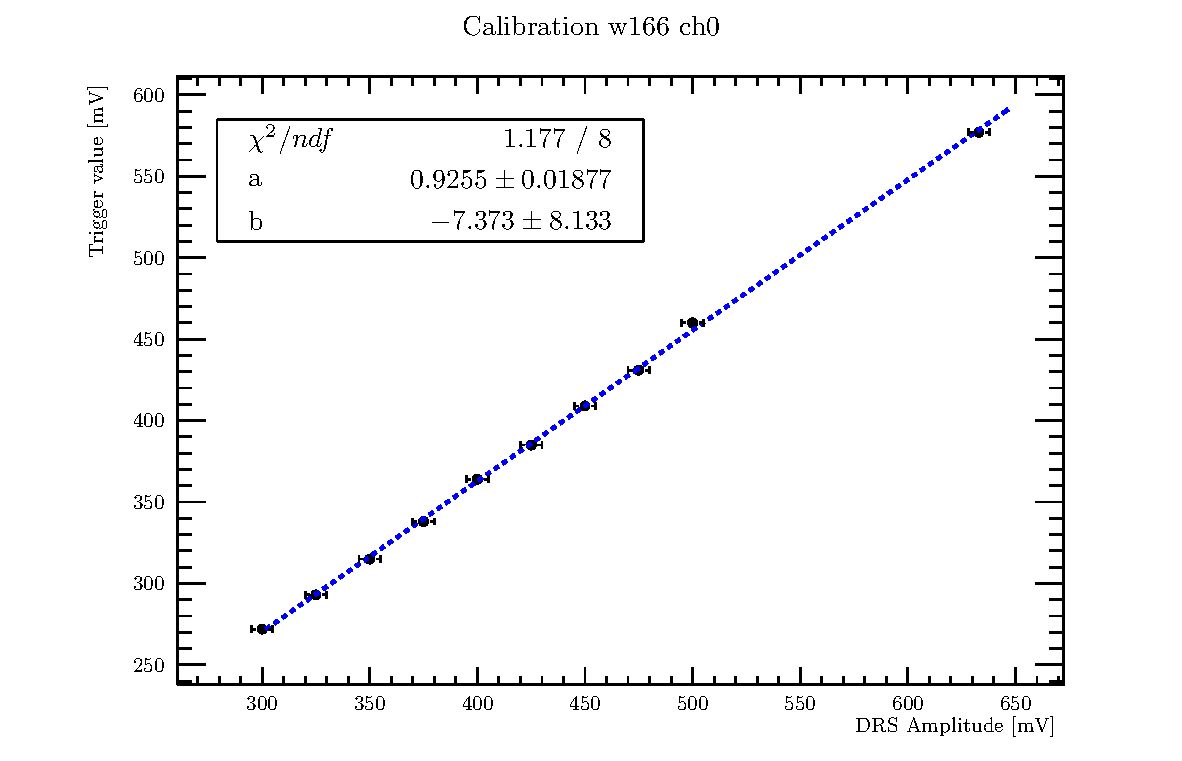
\includegraphics[scale=0.5]{figures/ch0.pdf}
			\caption{Channel 0.}
		\end{figure}  
\end{frame}

%==================================================================
				%SLIDE 5 - Channels calibration
%==================================================================

\begin{frame} [fragile]
\small
	\frametitle{Channels calibration}
    		\begin{figure}
		 \centering
			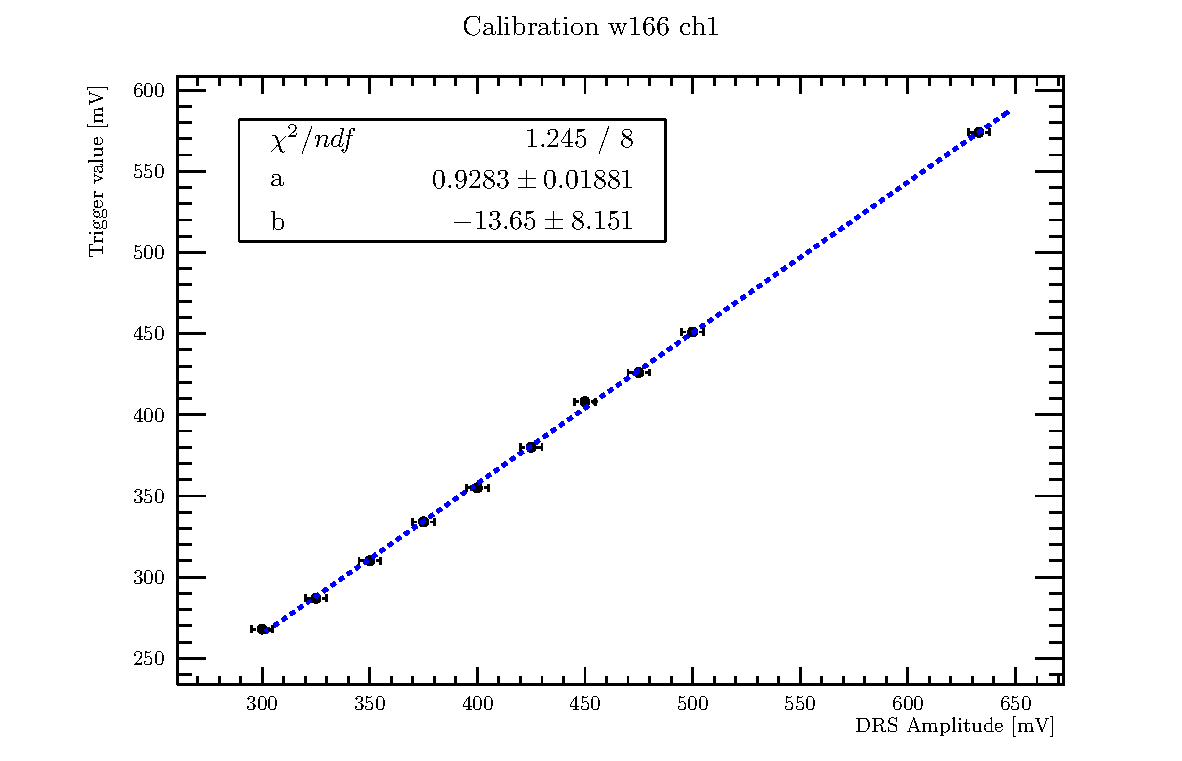
\includegraphics[scale=0.5]{figures/ch1.pdf}
			\caption{Channel 1.}
		\end{figure}  
\end{frame}

%==================================================================
				%SLIDE 5 - Channels calibration
%==================================================================

\begin{frame} [fragile]
\small
	\frametitle{Channels calibration}
    		\begin{figure}
		 \centering
			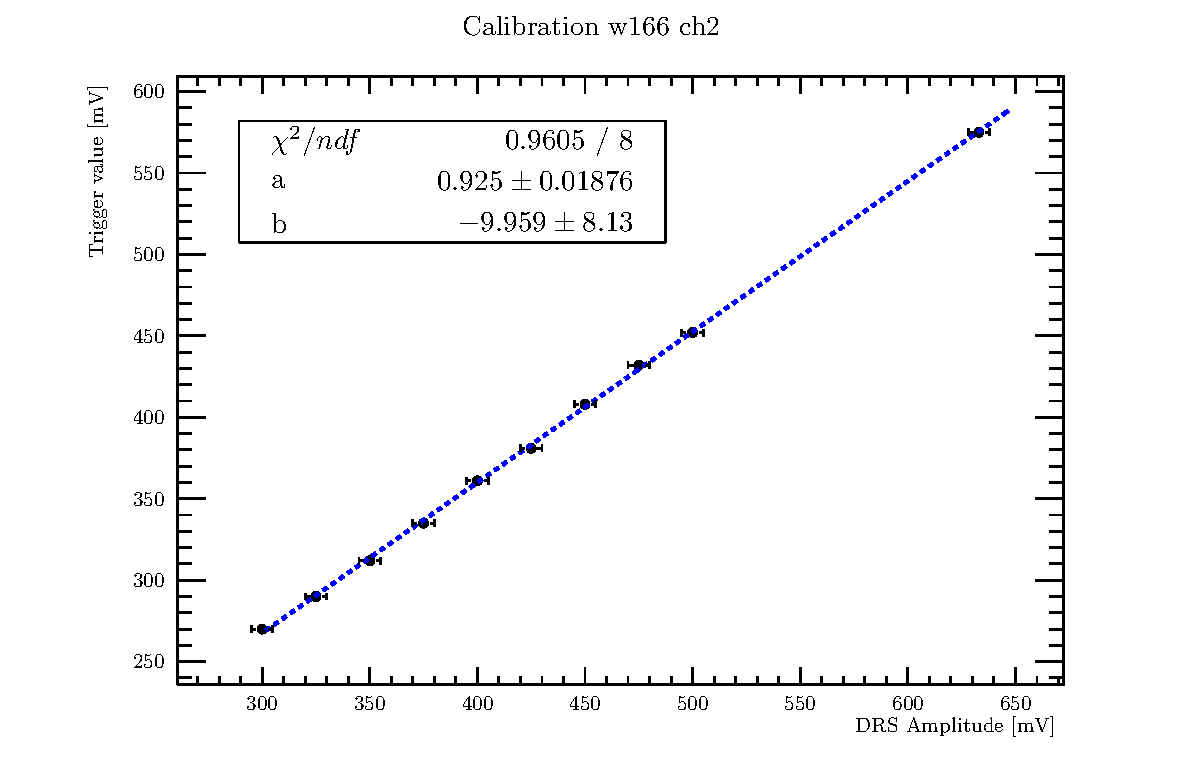
\includegraphics[scale=0.5]{figures/ch2.pdf}
			\caption{Channel 2.}
		\end{figure}  
\end{frame}

%==================================================================
				%SLIDE 5 - Channels calibration
%==================================================================

\begin{frame} [fragile]
\small
	\frametitle{Channels calibration}
    		\begin{figure}
		 \centering
			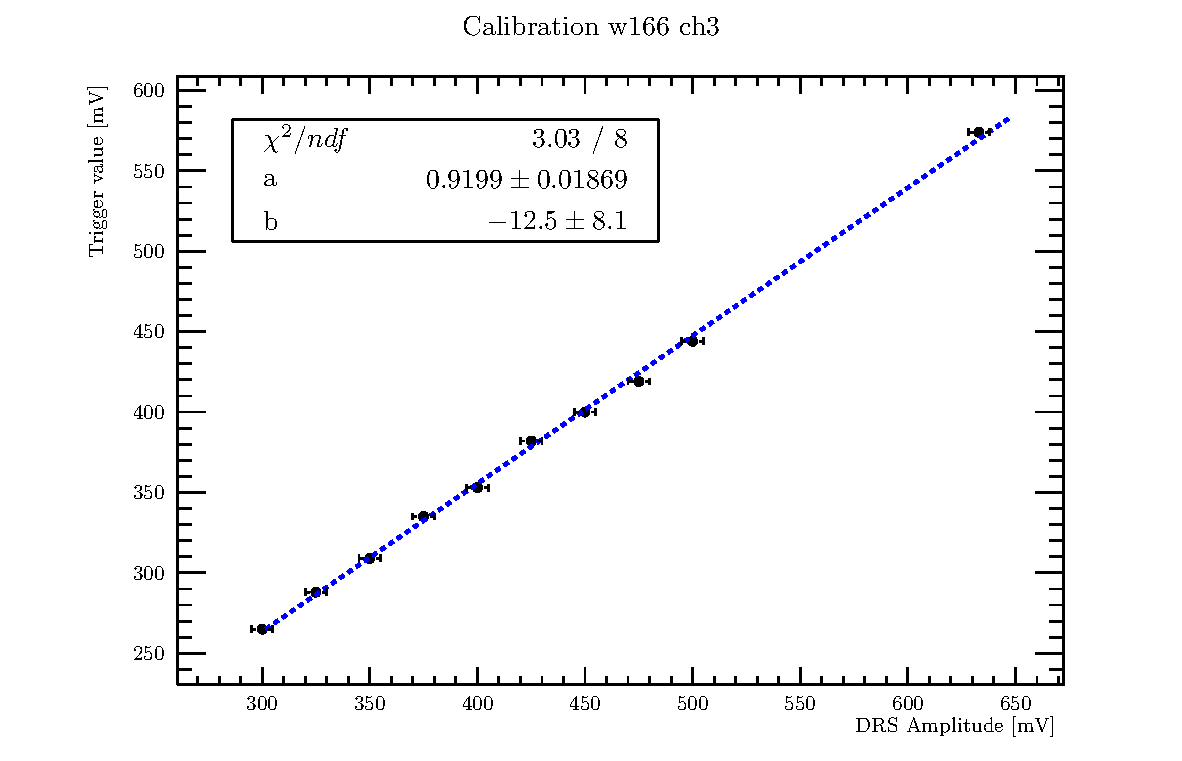
\includegraphics[scale=0.5]{figures/ch3.pdf}
			\caption{Channel 3.}
		\end{figure}  
\end{frame}

%==================================================================
				%SLIDE 5 - Channels calibration
%==================================================================

\begin{frame} [fragile]
\small
	\frametitle{Channels calibration}
    		\begin{figure}
		 \centering
			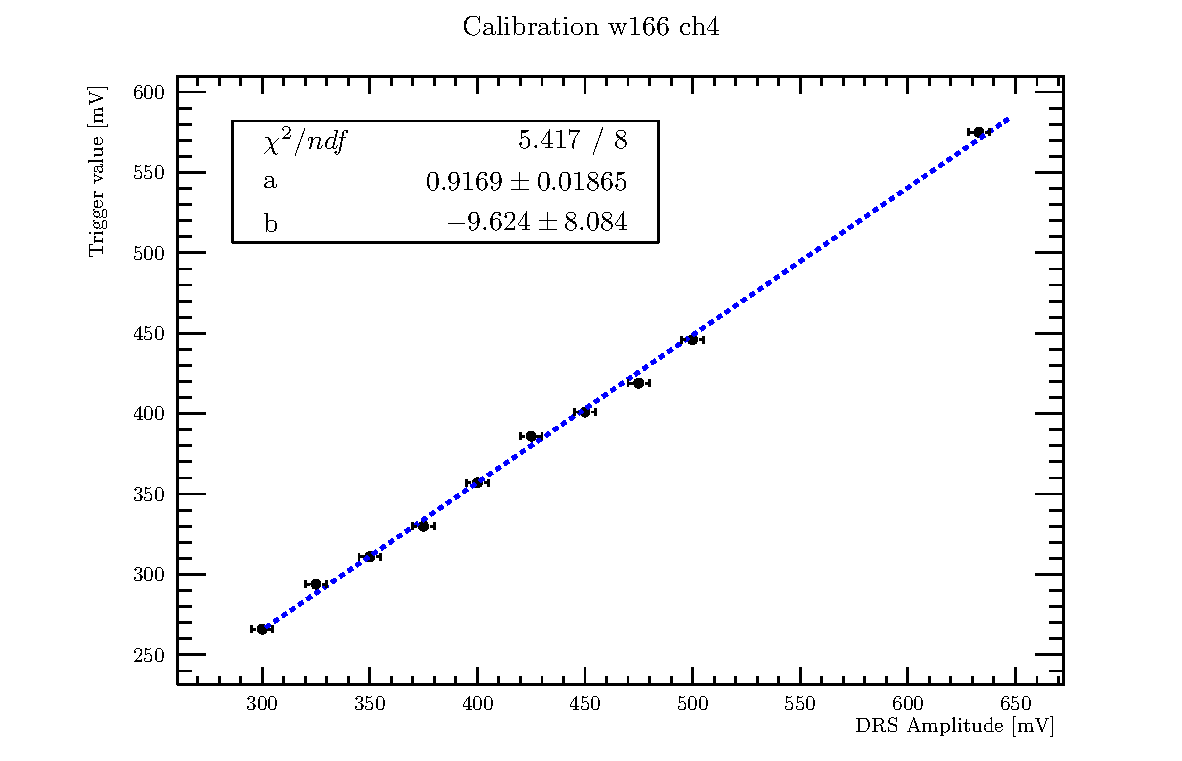
\includegraphics[scale=0.5]{figures/ch4.pdf}
			\caption{Channel 4.}
		\end{figure}  
\end{frame}

%==================================================================
				%SLIDE 5 - Channels calibration
%==================================================================

\begin{frame} [fragile]
\small
	\frametitle{Channels calibration}
    		\begin{figure}
		 \centering
			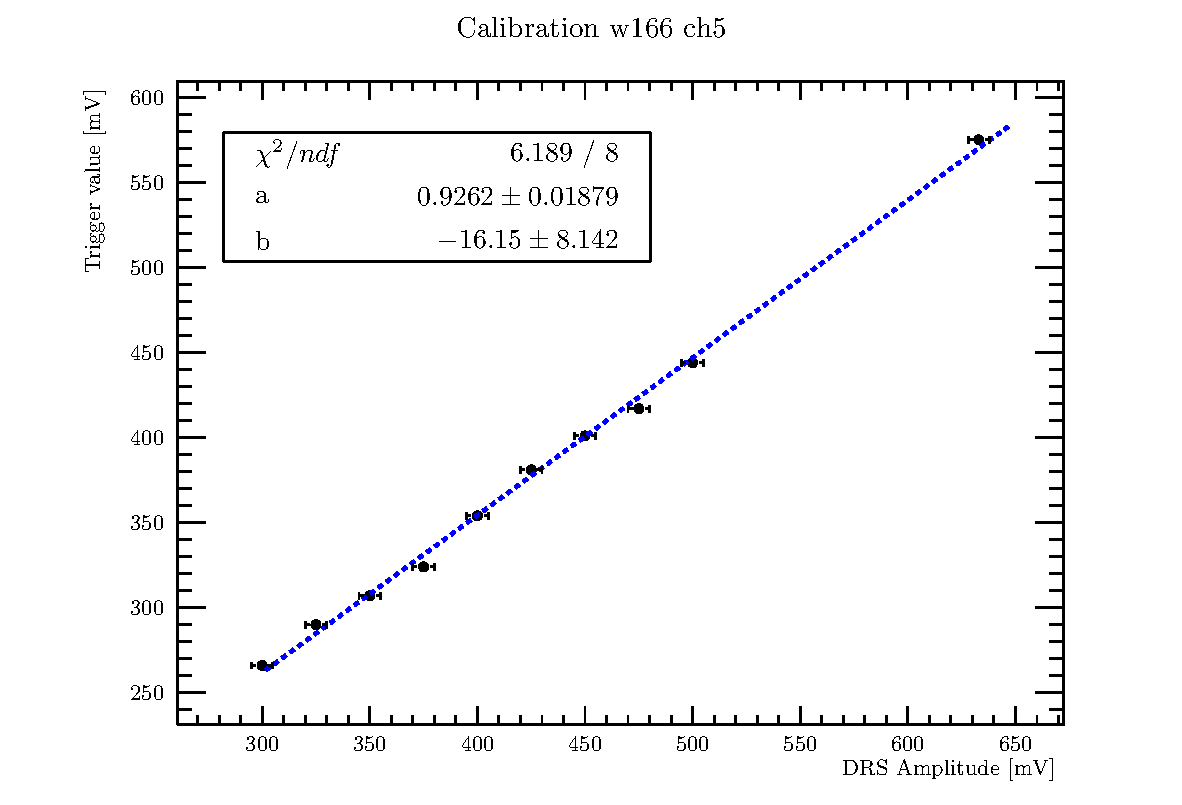
\includegraphics[scale=0.5]{figures/ch5.pdf}
			\caption{Channel 5.}
		\end{figure}  
\end{frame}

%==================================================================
				%SLIDE 5 - Channels calibration
%==================================================================

\begin{frame} [fragile]
\small
	\frametitle{Channels calibration}
    		\begin{figure}
		 \centering
			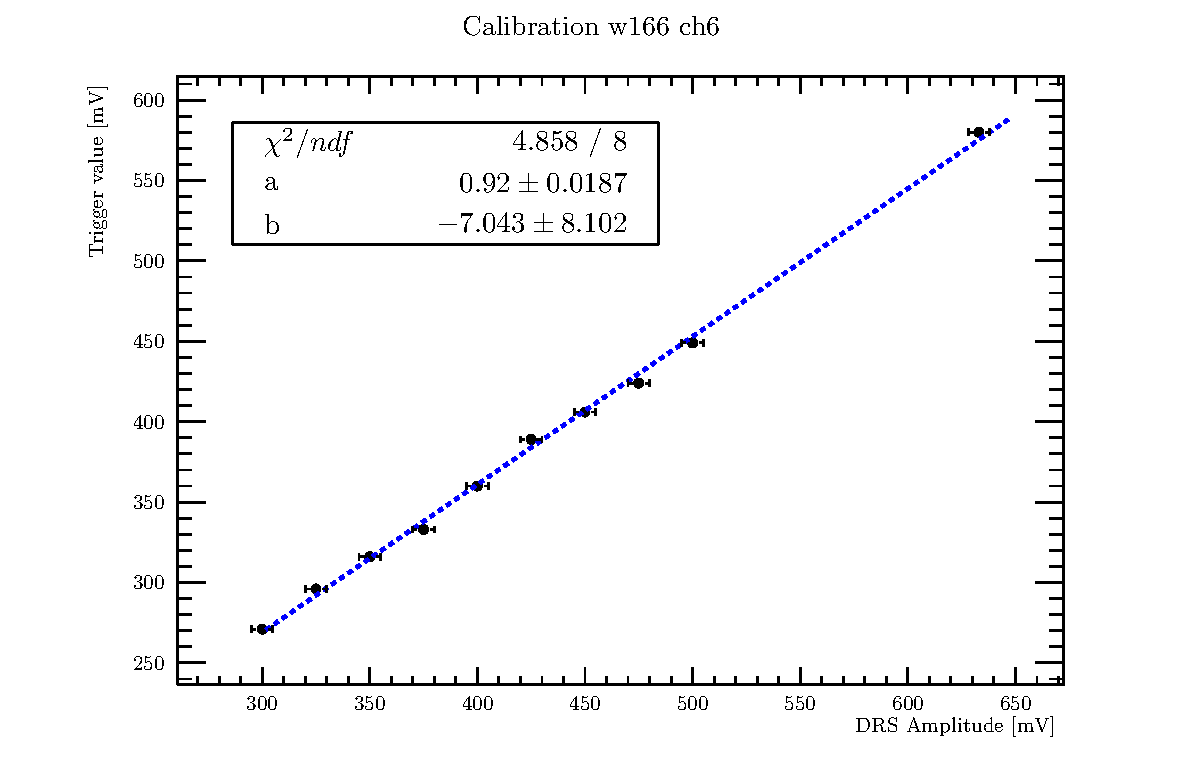
\includegraphics[scale=0.5]{figures/ch6.pdf}
			\caption{Channel 6.}
		\end{figure}  
\end{frame}

%==================================================================
				%SLIDE 5 - Channels calibration
%==================================================================

\begin{frame} [fragile]
\small
	\frametitle{Channels calibration}
    		\begin{figure}
		 \centering
			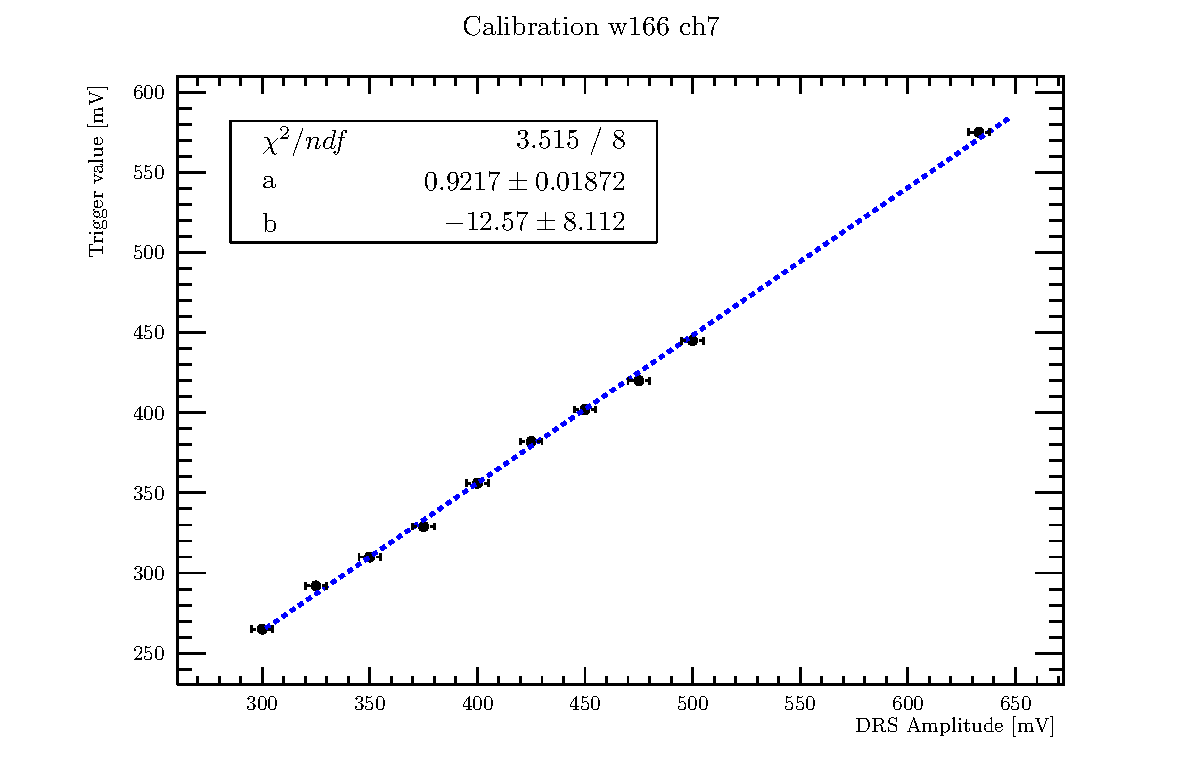
\includegraphics[scale=0.5]{figures/ch7.pdf}
			\caption{Channel 7.}
		\end{figure}  
\end{frame}

%==================================================================
				%SLIDE 5 - Channels calibration
%==================================================================

\begin{frame} [fragile]
\small
	\frametitle{Channels calibration}
    		\begin{figure}
		 \centering
			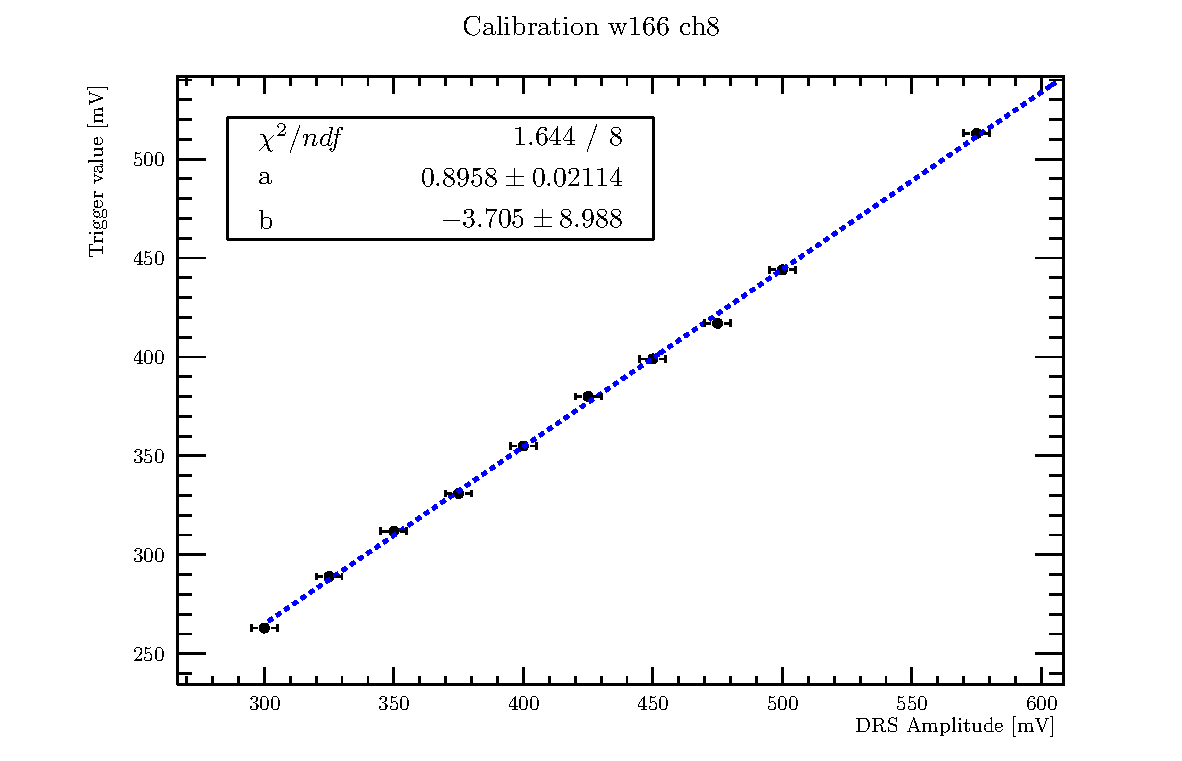
\includegraphics[scale=0.5]{figures/ch8.pdf}
			\caption{Channel 8.}
		\end{figure}  
\end{frame}

%==================================================================
				%SLIDE 5 - Channels calibration
%==================================================================

\begin{frame} [fragile]
\small
	\frametitle{Channels calibration}
    		\begin{figure}
		 \centering
			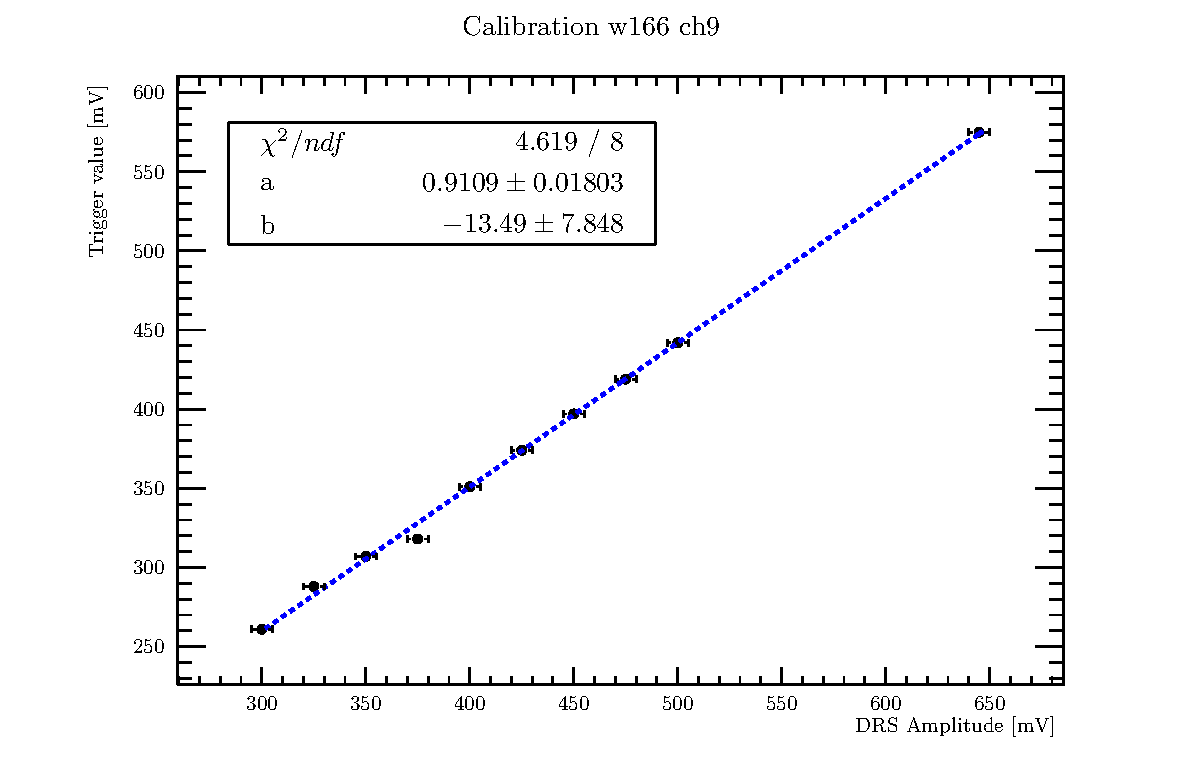
\includegraphics[scale=0.5]{figures/ch9.pdf}
			\caption{Channel 9.}
		\end{figure}  
\end{frame}

%==================================================================
				%SLIDE 5 - Channels calibration
%==================================================================

\begin{frame} [fragile]
\small
	\frametitle{Channels calibration}
    		\begin{figure}
		 \centering
			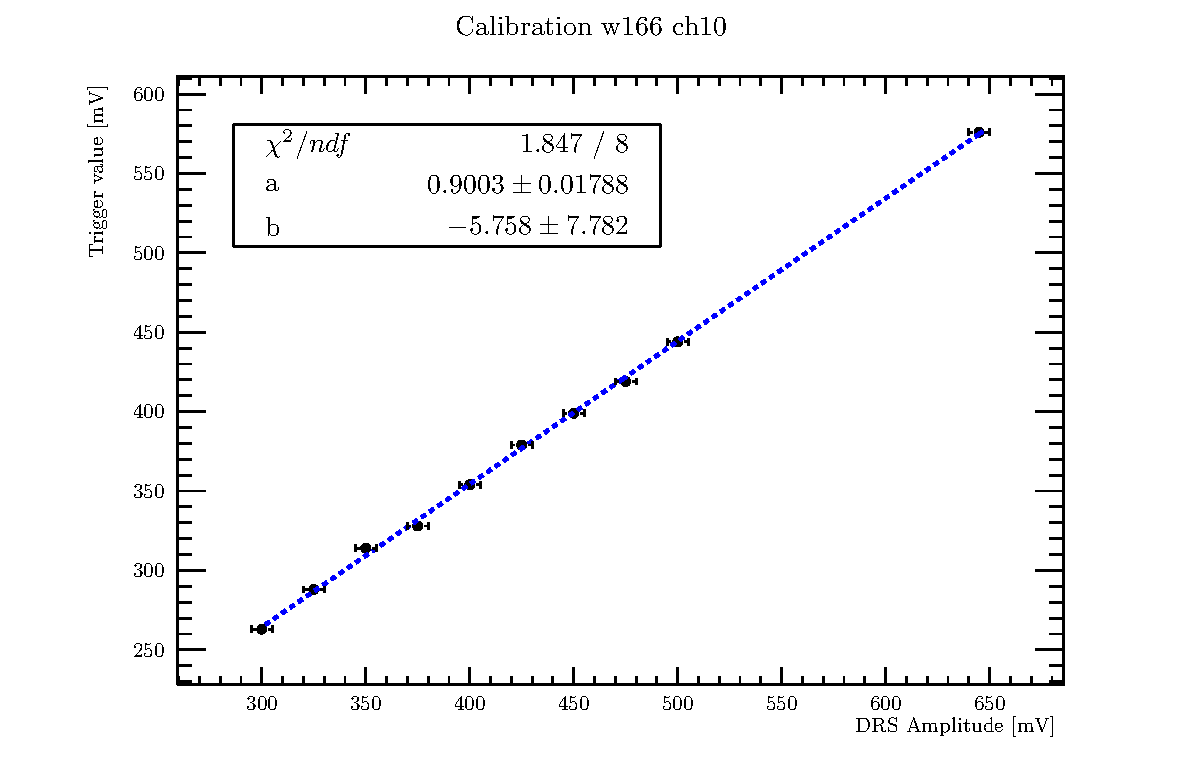
\includegraphics[scale=0.5]{figures/ch10.pdf}
			\caption{Channel 10.}
		\end{figure}  
\end{frame}

%==================================================================
				%SLIDE 5 - Channels calibration
%==================================================================

\begin{frame} [fragile]
\small
	\frametitle{Channels calibration}
    		\begin{figure}
		 \centering
			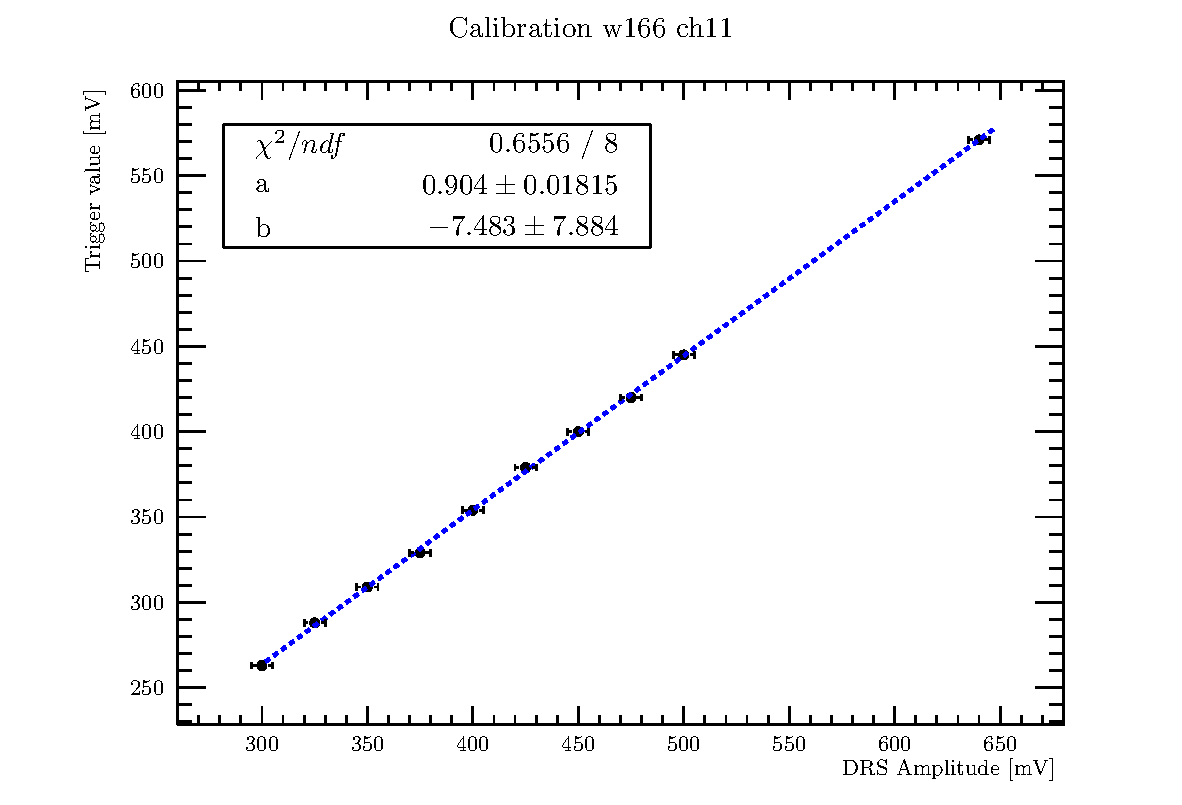
\includegraphics[scale=0.5]{figures/ch11.pdf}
			\caption{Channel 11.}
		\end{figure}  
\end{frame}



	
%==================================================================
						%SLIDE - thebibliography
%==================================================================

\begin{frame}
\frametitle{\refname}
   \begin{thebibliography}{9}
   \small
   

      \bibitem{BLANCATO} Antonella Alessandra Blancato
      \newblock \textit{Rischi da radiazione nei voli interplanetari}
      \newblock \emph{Tesi di Laurea}, 2007-2008
      

   \end{thebibliography}
\end{frame}
%==================================================================

\end{document}